\documentclass{beamer}
\usepackage[utf8]{inputenc}

\usepackage{amsmath}
\usepackage{graphicx}
\usepackage{url}
\usepackage{fancyvrb}
\usepackage{xcolor}

\usetheme{Boadilla}
\usecolortheme{whale}
\usepackage{lmodern}

\usepackage{listings}
\usepackage{color}

\definecolor{codegreen}{rgb}{0,0.6,0}
\definecolor{codegray}{rgb}{0.5,0.5,0.5}
\definecolor{codepurple}{rgb}{0.58,0,0.82}
\definecolor{backcolour}{rgb}{0.95,0.95,0.92}

\mode<presentation>

\definecolor{orange}{HTML}{BC2E07}

\usepackage{hyperref}
\hypersetup{
    colorlinks,
    linkcolor=orange,
    urlcolor=blue
}

\lstdefinestyle{mystyle}{
    language=C++,
    basicstyle=\ttfamily\footnotesize,
    backgroundcolor=\color{backcolour},
    commentstyle=\color{codegreen},
    keywordstyle=\color{magenta},
    numberstyle=\tiny\color{codegray},
    stringstyle=\color{codepurple},
    breakatwhitespace=false,
    breaklines=true,
    captionpos=b,
    keepspaces=true,
    numbers=left,
    numbersep=5pt,
    showspaces=false,
    showstringspaces=false,
    showtabs=false,
    tabsize=2
}

\title{Lab \# 5: More Control Statements}
\subtitle{EC-102 -- Computer Systems and Programming}

\author{Usman Ayub Sheikh}
\institute{School of Mechanical and Manufacturing Engineering (SMME), \\ National University of Sciences and Technology (NUST)}
\date{\today}

\begin{document}
\begin{frame}
    \titlepage
\end{frame}

\begin{frame}
    \frametitle{Outline}
        \tableofcontents
\end{frame}

\begin{frame}
    \frametitle{The \texttt{switch} Statement - Introduction}
    \section{More Decision Statements} % (fold)
    \label{sec:more_decision_statements}
    \subsection{The \texttt{switch} Statement} % (fold)
    \label{sub:the_switch_statement}
    \begin{columns}
        \column{0.5\textwidth}
        \begin{itemize}
            \item Large decision tree
            \item All the decisions depend on the value of the same variable
            \item May be used instead of nested \texttt{if...else} statement
        \end{itemize}
        \column{0.5\textwidth}
        \begin{figure}
            \centering
            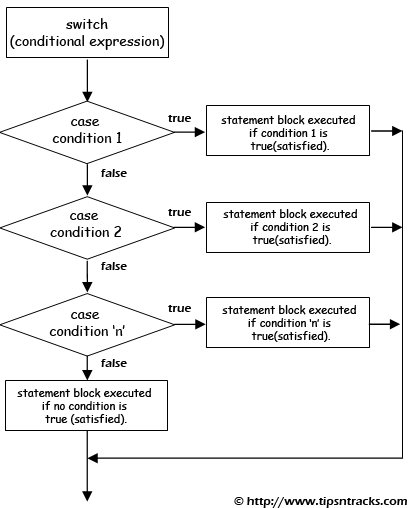
\includegraphics[scale=0.35]{switch}
        \end{figure}
    \end{columns}
\end{frame}

\begin{frame}[fragile]
    \frametitle{The \texttt{switch} Statement - Syntax}
    \begin{columns}
        \column{0.3\textwidth}
        \lstset{style=mystyle}
        \begin{lstlisting}
switch(n)
{
    case 1:
    statement 1;
    statement 2;
    break;

    case 2:
    statement 1;
    statement 2;
    break;

    case 3:
    statement;
    break;

    default:
    statement;
}
\end{lstlisting}
        \column{0.65\textwidth}
            \begin{itemize}
            \item The keyword \texttt{switch} is followed by a switch variable in parentheses (Line 1)
            \item Braces are used to delimit all \texttt{case} statements
            \item Each \texttt{case} keyword is followed by a constant which is not in parentheses but is followed by a colon (Lines 3, 8 and 13)
            \item The data type of the \texttt{case} constants should match that of the \texttt{switch} variable
            \item \texttt{default} keyword gives the switch construction a way to take an action if the value of the variable does not match any of the \texttt{case} constants (Line 17)
            \end{itemize}
    \end{columns}
\end{frame}

\begin{frame}
    \frametitle{The \texttt{break} Statement}
    \subsection{The \texttt{break} Statement} % (fold)
    \label{sub:the_break_statement}
    \begin{itemize}
        \item Causes the entire \texttt{switch} statement to exit
        \item Control goes to the first statement following the end of the \texttt{switch} contruction
    \end{itemize}
\end{frame}

\begin{frame}[fragile]
    \frametitle{Solved Example}
    \section{Solved Example} % (fold)
    \label{sec:solved_example}
    \begin{columns}
    \column{0.5\textwidth}
    \textbf{Algorithm}
    \begin{enumerate}
        \item Start
        \item Declare variable \texttt{grade}
        \item Read value of \texttt{grade}
        \item If grade is `A' then display `Excellent!'
        \item Else if grade is `B' or `C' then display `Well done'
        \item Else if grade is `D' then display `You passed'
        \item Else if grade is `F' then display `Better try again'
        \item Else display `Invalid grade'
        \item Stop
    \end{enumerate}
    \column{0.50\textwidth}
    \textbf{Flowchart}
    \begin{figure}
        \centering
        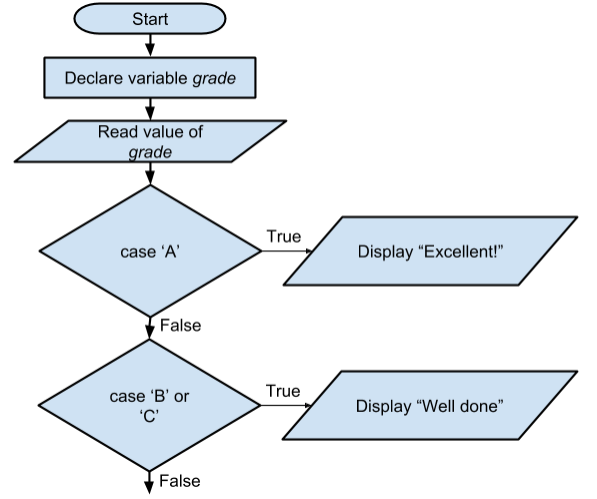
\includegraphics[scale=0.4]{pflow}
    \end{figure}
    \end{columns}
\end{frame}

\begin{frame} [fragile]
    \frametitle{Solved Example}
    \lstset{style=mystyle}
    \begin{lstlisting}
#include <iostream>
using namespace std;

int main ()
{
   char grade;
   cout << "Enter a grade (eg. A, B etc): ";
   cin >> grade;
   switch(grade)
   {
   case 'A' :
      cout << "Excellent!" << endl;
      break;
   case 'B' :
   case 'C' :
      cout << "Well done" << endl;
      break;
   case 'D' :
      cout << "You passed" << endl;
      break;
\end{lstlisting}
\end{frame}

\begin{frame} [fragile]
    \frametitle{Solved Example}
    \lstset{style=mystyle}
    \begin{lstlisting} [firstnumber=21]
    case 'F' :
        cout << "Better try again" << endl;
        break;
    default :
        cout << "Invalid grade" << endl;
    }
    return 0;
}
\end{lstlisting}
\end{frame}

\begin{frame}
    \frametitle{Exercise}
    \section{Exercise} % (fold)
    \label{sec:exercise}
    Develop a basic calculator using \texttt{switch} statement which is capable of performing addition, subtraction, multiplication and division
    \begin{itemize}
        \item Ask the user to enter two numbers and the type of arithmetic operation to be performed
        \item Use \texttt{char} data type for the variable handling the operator
    \end{itemize}
\end{frame}
\end{document}